\section*{Problemas}

\subsection*{Enunciados de los problemas}

% Recordar
\begin{problema}
	\label{prob:f690fbe}
	Escribir los términos de cada una de las siguientes sumas:
	\begin{enumerate}
		\item $\displaystyle\sum_{j=0}^{6}X_{j}=$
		\item $\displaystyle\sum_{k=1}^{4}\left( Y_{k}-3 \right)^{2}=$
		\item $\displaystyle\sum_{k=1}^{N}a=$
		\item $\displaystyle\sum_{n=2}^{5}{f_{n}}X_{n}= $
		\item $\displaystyle\sum_{m=0}^{3}\left( X_{m}-a \right)=$
	\end{enumerate}
\end{problema}

% Comprender
\begin{problema}
	\label{prob:0b934f5}
	Demuestre que la suma de las desviaciones $d_{1},d_{2},...,d_{N}$ de $X_{1},X_{2},...,X_{N}$ usando como pivote su propia media $\bar{X}$ es igual a cero, y explique por qué esta propiedad justifica describir a la media aritmética como el "centro de gravedad" de un conjunto de datos.
\end{problema}

% Aplicar
\begin{problema}
	\label{prob:0c7ed43}
	Usando la distribución de frecuencias de las estaturas que se presenta en la siguiente tabla, halle la estatura media de 100 estudiantes de cierta universidad.
	\begin{figure}[ht]
		\centering
		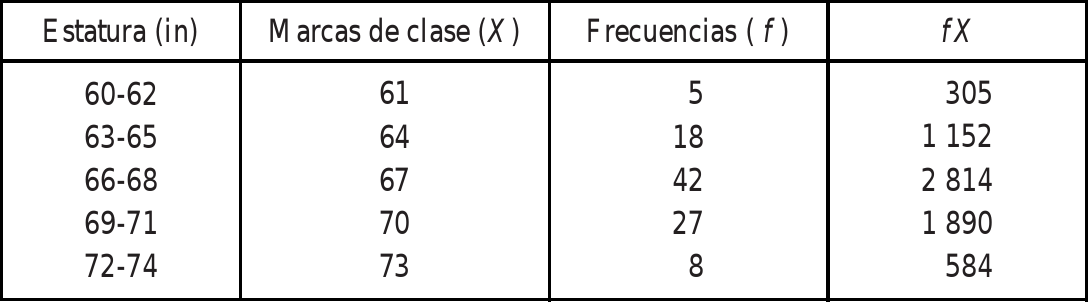
\includegraphics[width=10cm,keepaspectratio=true]{./images/tab0301.png}
		\label{tab:1.2.1-medidas}
	\end{figure}
\end{problema}

% Analizar
\begin{problema}
	\label{prob:08f4f21}
	Si las desviaciones de $N$ números $X_{1},..,X_{N}$ respecto a un \emph{pivote} arbitrario $P$ están dadas por $d_{i}=X_{i}-P, \; i=1,...,N$, demuestre algebraicamente que
	\begin{align}
		\bar{X}=P+\dfrac{\sum d_{i}}{N},
	\end{align}
	y verifique con este resultado que la fórmula anterior es válida sin importar qué valor de $P$ se elija.
\end{problema}

% Evaluar
\begin{problema}
	\label{prob:ced3c3b}
	Utilice la marca de la clase central como pivote y el método de codificación por cambio de escala y origen ($u_i = (X_i-P)/c$) para recalcular la estatura media de los 100 estudiantes del Problema \ref{prob:0c7ed43}. Compare el resultado y el esfuerzo aritmético contra el cálculo directo, y evalúe en qué situaciones (tamaño de la tabla, amplitud de clase, recursos de cómputo disponibles) conviene preferir el método codificado sobre el método directo.
\end{problema}

% Crear
\begin{problema}
	\label{prob:32476e7}
	Un analista registra el tiempo de respuesta (en milisegundos) de 60 solicitudes a un servidor web, agrupadas en la siguiente tabla de frecuencias:
	\begin{center}
		\begin{tabular}{cccc}
			\hline
			Intervalo (ms) & Marca de clase $X_i$ & Frecuencia $f_i$ & Frec. acumulada $F_i$ \\
			\hline
			10--19 & 14.5 & 6  & 6 \\
			20--29 & 24.5 & 14 & 20 \\
			30--39 & 34.5 & 22 & 42 \\
			40--49 & 44.5 & 12 & 54 \\
			50--59 & 54.5 & 6  & 60 \\
			\hline
		\end{tabular}
	\end{center}
	Diseñe la solución completa: calcule (a) el tiempo medio de respuesta $\bar{X}$ usando la marca de clase, y (b) el tiempo mediano de respuesta mediante interpolación lineal en la clase que contiene a la observación número $N/2=30$.
\end{problema}

\subsection*{Soluciones detalladas}

% Recordar
\begin{solproblema}[prob:f690fbe]
	Desarrollando término a término cada sumatoria según los índices indicados:
	\begin{enumerate}
		\item $\displaystyle\sum_{j=0}^{6}X_{j} = X_{0} + X_{1} + X_{2} + X_{3} + X_{4} + X_{5} + X_{6}$
		\item $\displaystyle\sum_{k=1}^{4}\left( Y_{k}-3 \right)^{2} = (Y_{1}-3)^{2} + (Y_{2}-3)^{2} + (Y_{3}-3)^{2} + (Y_{4}-3)^{2}$
		\item $\displaystyle\sum_{k=1}^{N}a = \underbrace{a + a + \cdots + a}_{N \text{ veces}} = N \cdot a$
		\item $\displaystyle\sum_{n=2}^{5}{f_{n}}X_{n} = f_{2}X_{2} + f_{3}X_{3} + f_{4}X_{4} + f_{5}X_{5}$
		\item $\displaystyle\sum_{m=0}^{3}\left( X_{m}-a \right) = (X_{0}-a) + (X_{1}-a) + (X_{2}-a) + (X_{3}-a)$
	\end{enumerate}
\end{solproblema}

% Comprender
\begin{solproblema}[prob:0b934f5]
	Sea $d_{i} = X_{i} - \bar{X}$. Sumando para todos los $N$ elementos del conjunto:
	\begin{align}
		\sum_{i=1}^{N} d_{i} &= \sum_{i=1}^{N} (X_{i} - \bar{X}) = \sum_{i=1}^{N} X_{i} - \sum_{i=1}^{N} \bar{X}.
	\end{align}
	Como $\bar{X}$ es una constante respecto al índice de sumatoria $i$, $\sum_{i=1}^{N} \bar{X} = N\bar{X}$. Además, por definición de media aritmética, $\sum_{i=1}^{N} X_{i} = N\bar{X}$. Sustituyendo ambos términos:
	\begin{align}
		\sum_{i=1}^{N} d_{i} = N\bar{X} - N\bar{X} = 0.
	\end{align}
	Esta propiedad justifica la interpretación física de la media como "centro de gravedad": así como el punto de equilibrio de un sistema de masas es aquel donde los momentos a ambos lados se cancelan, la media es el único pivote donde las desviaciones positivas y negativas de los datos se cancelan exactamente entre sí.
\end{solproblema}

% Aplicar
\begin{solproblema}[prob:0c7ed43]
	A partir de la tabla, determinamos el punto medio o marca de clase ($X_{i}$) para cada intervalo de estatura (en pulgadas) y multiplicamos por su frecuencia $f_{i}$:
	\begin{itemize}
		\item Intervalo 60--62: $X_{1} = 61$, $f_{1} = 5 \implies f_{1}X_{1} = 305$
		\item Intervalo 63--65: $X_{2} = 64$, $f_{2} = 18 \implies f_{2}X_{2} = 1152$
		\item Intervalo 66--68: $X_{3} = 67$, $f_{3} = 42 \implies f_{3}X_{3} = 2814$
		\item Intervalo 69--71: $X_{4} = 70$, $f_{4} = 27 \implies f_{4}X_{4} = 1890$
		\item Intervalo 72--74: $X_{5} = 73$, $f_{5} = 8 \implies f_{5}X_{5} = 584$
	\end{itemize}
	Sumando las frecuencias y los productos:
	\begin{align}
		N &= \sum f_{i} = 5 + 18 + 42 + 27 + 8 = 100 \\
		\sum f_{i}X_{i} &= 305 + 1152 + 2814 + 1890 + 584 = 6745
	\end{align}
	Por lo tanto, la estatura media es:
	\begin{align}
		\bar{X} = \dfrac{6745}{100} = 67.45 \text{ pulgadas.}
	\end{align}
\end{solproblema}

% Analizar
\begin{solproblema}[prob:08f4f21]
	Partimos de la definición de desviación respecto al pivote: $d_{i} = X_{i} - P$. Despejando la variable original tenemos $X_{i} = P + d_{i}$. Sumando desde $i=1$ hasta $N$ en ambos lados de la igualdad:
	\begin{align}
		\sum_{i=1}^{N} X_{i} &= \sum_{i=1}^{N} (P + d_{i}) = \sum_{i=1}^{N} P + \sum_{i=1}^{N} d_{i} = N \cdot P + \sum_{i=1}^{N} d_{i}.
	\end{align}
	Dividiendo toda la expresión entre $N$:
	\begin{align}
		\dfrac{\sum_{i=1}^{N} X_{i}}{N} &= \dfrac{N \cdot P}{N} + \dfrac{\sum_{i=1}^{N} d_{i}}{N} \implies \bar{X} = P + \dfrac{\sum_{i=1}^{N} d_{i}}{N}.
	\end{align}
	Esta derivación no impuso ninguna restricción sobre el valor de $P$: es válida para \emph{cualquier} pivote elegido, ya sea $P=0$, la media de otra muestra, o un valor arbitrario, siempre que $\sum d_i$ se recalcule respecto a ese mismo $P$. Esto es justamente lo que verifica numéricamente el resultado invariante $\bar{X}=9.375$ al usar $P=9$ o $P=20$ sobre el mismo conjunto de datos.
\end{solproblema}

% Evaluar
\begin{solproblema}[prob:ced3c3b]
	La marca de clase del intervalo central (66--68) es $P = 67$ pulgadas. Como las clases tienen un ancho constante $c = 3$ pulgadas, usamos la variable codificada $u_{i} = \dfrac{X_{i} - P}{c}$:
	\begin{itemize}
		\item Cl. 60--62 ($X_{1}=61$): $u_{1} = \frac{61-67}{3} = -2 \implies f_{1}u_{1} = 5(-2) = -10$
		\item Cl. 63--65 ($X_{2}=64$): $u_{2} = \frac{64-67}{3} = -1 \implies f_{2}u_{2} = 18(-1) = -18$
		\item Cl. 66--68 ($X_{3}=67$): $u_{3} = \frac{67-67}{3} = 0 \implies f_{3}u_{3} = 42(0) = 0$
		\item Cl. 69--71 ($X_{4}=70$): $u_{4} = \frac{70-67}{3} = 1 \implies f_{4}u_{4} = 27(1) = 27$
		\item Cl. 72--74 ($X_{5}=73$): $u_{5} = \frac{73-67}{3} = 2 \implies f_{5}u_{5} = 8(2) = 16$
	\end{itemize}
	Sumando las frecuencias por el código, $\sum f_{i}u_{i} = -10 - 18 + 0 + 27 + 16 = 15$. Aplicando la fórmula abreviada de la media con cambio de escala y origen:
	\begin{align}
		\bar{X} = P + c\left( \dfrac{\sum f_{i}u_{i}}{N} \right) = 67 + 3\left( \dfrac{15}{100} \right) = 67.45 \text{ pulgadas,}
	\end{align}
	idéntico al resultado directo del Problema \ref{prob:0c7ed43}. En cuanto al esfuerzo aritmético, el método codificado reemplaza productos de números grandes (marca de clase $\times$ frecuencia, valores de dos y tres cifras) por productos de enteros pequeños ($-2$ a $2$), lo cual reduce el riesgo de error de cálculo manual. Sin embargo, con software o calculadoras estadísticas la ventaja desaparece casi por completo, ya que ambos métodos son igual de rápidos de ejecutar. El método codificado conviene, entonces, principalmente en cálculo manual con tablas grandes o amplitud de clase constante, no como sustituto sistemático en un flujo de trabajo computarizado.
\end{solproblema}

% Crear
\begin{solproblema}[prob:32476e7]
	\textbf{(a) Media aritmética.} Multiplicando cada marca de clase por su frecuencia:
	\begin{align}
		\sum f_iX_i = 6(14.5)+14(24.5)+22(34.5)+12(44.5)+6(54.5) = 87+343+759+534+327 = 2050.
	\end{align}
	Con $N=60$:
	\begin{align}
		\bar{X} = \dfrac{2050}{60} \approx 34.17 \text{ ms.}
	\end{align}
	\textbf{(b) Mediana por interpolación.} Buscamos la clase que contiene a la observación $N/2=30$: la frecuencia acumulada llega a $F=20$ al final de la clase 20--29 y a $F=42$ al final de la clase 30--39, así que la clase mediana es 30--39, con límite real inferior $L_m=29.5$, frecuencia acumulada anterior $F_{m-1}=20$, frecuencia de la clase $f_m=22$ y amplitud $c=10$:
	\begin{align}
		Med = L_m + \left( \dfrac{N/2 - F_{m-1}}{f_m} \right)c = 29.5 + \left( \dfrac{30-20}{22} \right)(10) = 29.5 + 4.55 = 34.05 \text{ ms.}
	\end{align}
	La media ($34.17$ ms) y la mediana ($34.05$ ms) resultan muy cercanas entre sí, lo cual es consistente con una distribución de tiempos de respuesta razonablemente simétrica alrededor de la clase central.
\end{solproblema}
